

\begin{document}
    \chapter{Introduction}
    \justifying
    \acrlong{av} (\acrshort{av}) perceives the operating environment using an array of sensors and navigate through any scenario without any human intervention. Though the development of \acrshort{av} is a highly sought-after challenge by many researchers and companies around the world. There are still many open questions surrounding the safety of the usage of \acrshort{av}. The safety issues stems from various stages in \acrshort{av} software pipeline as shown in Figure \ref{fig:ac_stack}.
    
    \begin{figure}[H]
        \centering
        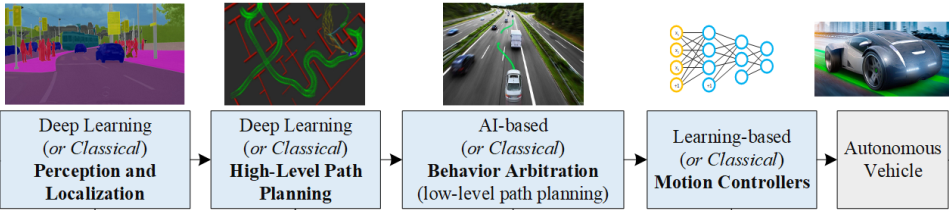
\includegraphics[scale=0.8]{images/Autonomous Driving stack.PNG}
        \caption[Autonomous Driving Stack]{Autonomous driving stack adapted from the works of \citet[pg.4]{Grigorescu2020}. In the first stage, the operating environments are perceived and the agents are localized the information from this stage is used in the second stage to perform safe-path planning. The output from the path planning stage is the main input for lateral and longitudinal controllers to safely navigate through the complex world around them. }
        \label{fig:ac_stack}
    \end{figure}
    
    A dependable perception is very important for the safe operation of \acrshort{av} as the motion and path planning algorithms have heavily relied on the accurate localization of the objects in the operating environment. To extract the information needed for the safe operation of \acrshort{av} \acrlong{dnn} (\acrshort{dnn}) are used. Since the operating environment is an open set \footnote{The samples present during deployment can vary from the training dataset}, the ability to detect whether the sample is present in the training set helps in the safe implementations of \acrshort{av}.
    
    \acrshort{dnn} which are trained discriminatively achieved best performances in tasks like speech recognition \citep{klosowski}, object detection \citep{DeepODReview} and image classification \citep{Voulodimos}. Object detection is one of the tasks that is revolutionized with the application of \acrlong{cnn} (\acrshort{cnn}) based DNNs \citep{DeepODReview}. It answers the following questions: 
    \begin{enumerate}
        \item what is in an image?
        \item where is it?
        \item how confident is the model in the detections?
    \end{enumerate}
    Despite their imposing performance, \acrshort{dnn} based models are proved to be resulting in overconfident predictions when the model encounters data that is different from the limited domain of expected inputs due to noise, adversarial corruptions, or other changes in semantic distribution. In this work, we concentrate on the latter type of data often referred to as being \acrlong{ood} (\acrshort{ood}) inputs \citep{goodfellow2014explaining, DNNFooled}. In the case of object detection, we consider the input is \acrshort{ood} if: 
    
    \begin{enumerate}
        \item Input is outside the semantic space formed by the images used for training the perception algorithm.
        \item Input consists of objects which are not used in training but have features closer to the object of interest.
    \end{enumerate}

    To illustrate this failure as shown in Figure \ref{fig:3}, let us consider a model trained on Common Object in Context (COCO) object detection dataset \citep{COCO_Dataset}. We assume that the dataset is sampled from a distribution $p(X)$ at training time, the samples from the distribution $p(X)$ are considered to be in-distribution samples. Training an object detection model refers to modifying the model parameters thereby enabling the model to localize the objects in the image and classifying them into the object of interest. When the model is made to perform inference on the input sampled from \acrlong{idd} (\acrshort{idd}) \citep{Varma2019IDDAD} which consists of novel objects like Auto-Rickshaw that are not present in the training dataset. As illustrated in Figure \ref{fig:1}, the network detects the novel object wrongly with a high probability of 81\%. Figure \ref{fig:2} represents another \acrshort{ood} sample collected during a rainy day and the model couldn't detect the objects that are present in the image but detected a Dog that is not presented in the scene. 
    
        \begin{figure}[!htbp]
            \centering
          \subcaptionbox{False Positive detection\label{fig:1}}{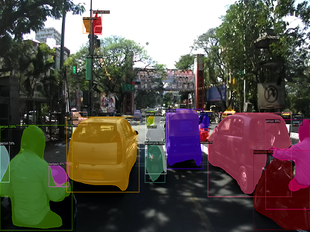
\includegraphics[scale=0.75]{images/False_Positive.png}}%\hspace{1em}
          \subcaptionbox{False Negative detection\label{fig:2}}{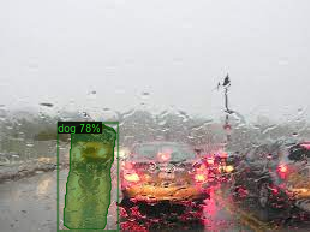
\includegraphics[scale=0.75]{images/False_Negative.png}}
          \caption[Sample False Positive and False Negative detections]{The sample image in Figure \ref{fig:1} represents False Positive detection in which an auto-rickshaw marked in blue is detected and classified as a car and Figure \ref{fig:2} represents False Negative detection in which cars are present in the scene but are not detected.}
          \label{fig:3}
        \end{figure}
    
    \section{Motivation}
        The inherent behavior of \acrshort{dnn} in providing over-confident results when provided with \acrshort{ood} samples is unsolicited in safety-critical applications like medical diagnosis and autonomous driving. One such \acrshort{ood} input scenario is faced in Brazil by a Tesla vehicle operating in Autopilot mode \citep{Gustavo2019}, where a boy wearing an orange reflective (high-vis) jacket is detected and classified as an orange traffic cone. This erroneous behavior is dangerous since the true class of the input belongs to a movable object while it's classified to be an immovable object. This false detection further results in faulty predictions from motion prediction and planning algorithms which might result in serious injuries or fatalities.
         
        Detecting and classifying this \acrshort{ood} samples results in the safe implementation of \acrshort{dnn} based object detection models where intentional or unintentional novel inputs may result in errors that might lead to catastrophic failures. \acrlong{av} (\acrshort{av}) development is one research area that benefits from the implementation of such \acrshort{ood} methods because of change in weather conditions, illumination levels, and also because of the novelty present in the semantics of the objects on the road. Detecting and localizing the \acrshort{ood} object present in the scene would help in better planning or fallback strategy.

    \section{Challenges and Difficulties}
        \begin{itemize}
            \item The majority of \acrshort{ood} detection methods proposed to date are designed entirely for object classification tasks. These methods proposed for object classification are not entirely adaptable to object detection tasks.
            \item The design philosophy of object detection problem includes foreground and background class. Background class is not generally included in training but should not be explicitly classified as a \acrshort{ood} data. The task of classifying between background class and \acrshort{ood} class is arduously challenging.
            \item Current available benchmarks are primarily proposed for evaluating \acrshort{ood} methods in classification and are comprised of small and simple datasets like CIFAR \cite{CIFAR}. Approaches proposed using these benchmarks make them non-transferable to complex environments or datasets.
        \end{itemize}


    \section{Problem Statement}
        In this work, we study the problem of out-of-distribution inputs in object detection tasks trained in a supervised setting. In particular, our task is to train a model using a dataset collected on the urban environment in clear weather and evaluate different \acrshort{ood} detection methods to detect objects in images sampled from \acrshort{ood} dataset.
        
        The task formulation of our problem is to train a \acrshort{dnn} model $M$ to perform regression task to extract the bounding box details together with a classification task to classify the type of object present in the image. We also employ another method or model to classify or quantify whether the input is \acrshort{ood} , we denote the model as $M_{ood}$. The deep learning model is trained using a dataset denoted by $D_{train}$ and validated on a dataset denoted by $D_{val}$ consisting of both \acrlong{id} (\acrshort{id}) and \acrshort{ood} samples, $D_{val}=D_{in-val} \bigcup D_{out-val}$. Finally, we test our model for benchmarking purposes on another dataset $D_{test}$, which is composed of both in-distribution and \acrshort{ood} samples $D_{test}=D_{in-test} \bigcup D_{out-test}$. Hence, an experiment $E$ composes of {$M$, $M_{ood}$, $D_{train}$, $D_{in-val}$,  $D_{out-val}$, $D_{in-test}$, $D_{out-test}$}. 
        
        The OOD detector should be able to produce a score which we refer to as \textbf{\textit{Novelty Score (NS)}}. NS can be a distance metric, a class-dependent probabilistic value, an entropy value or a descriptive statistic value based on the choice of the \acrshort{ood} method. Based on the method-specific score NS produced and a pre-defined threshold ($\delta$) the \acrshort{ood} can be posed as a binary classification problem. A sample can be classified as \acrshort{id} or \acrshort{ood} as shown in Equation \ref{id_vs_ood}.
        
        \begin{equation}
            X=
            \begin{cases}
              \text{\acrlong{id}}, & \text{if}\ NS \geq \delta \\
              \text{\acrlong{ood}}, & \text{otherwise} 
            \end{cases}
            \label{id_vs_ood}
        \end{equation}
        
        The behavior of the novelty score based on various inputs to the model is shown in Figure \ref{fig:OD2_features}
        
        \begin{figure}[H]
            \centering
            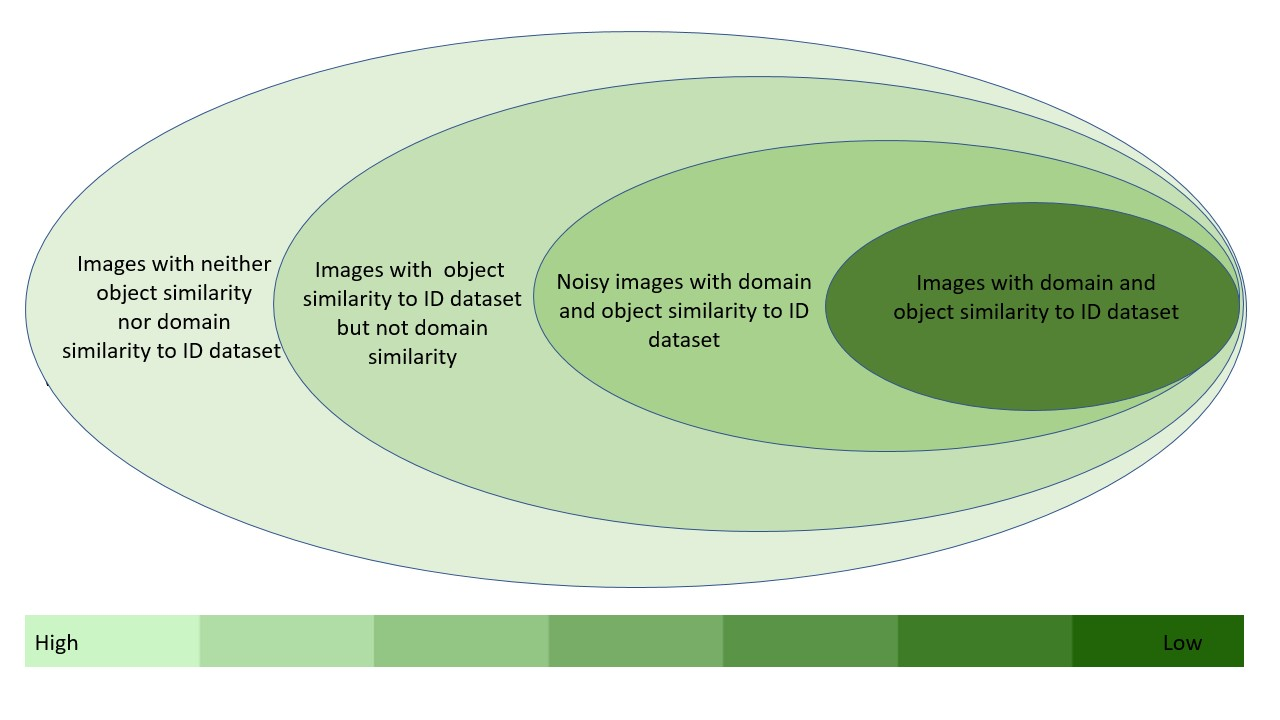
\includegraphics[scale=0.39]{images/Slide2.jpg}
            \caption[Novelty Score behavior]{Expected behavior of novelty score based on the nature of the \acrshort{ood} input}
            \label{fig:OD2_features}
        \end{figure}
        
        For \acrshort{ood} dataset, as proposed by \citet{Cao2020} three distinct out-of-distribution categories are considered
        \begin{itemize}
            \item Dataset from a different domain. For example, data that is collected in an urban environment is considered as \acrshort{id}. While, the dataset collected in remote environment is used as \acrshort{ood} dataset.
            \item Dataset with poor quality features. For example, data collected in an environment with poor illumination, rain and snowing conditions.
            \item Dataset with inputs that are neither used nor prominent in the training data. For example, using KITTI dataset \citep{KITTI2012} as an in-distribution dataset and using \acrshort{idd} \citep{Varma2019IDDAD} which consists of novel unseen classes as \acrshort{ood} dataset.
        \end{itemize}
\end{document}
